\section{通过漫画理解}

\emoji{l_sena} 
大家好.

习惯阅读幻日辞典的方法了么?

今天我们来借助字典读真正的Arka文本吧.


\emoji{x_sena} 
哇哦。真是实践编的感觉呢σ(°ー\^{}*)

so,要解读什么?虽然掌握了语法,也会使用词典,但是那种特别难的小说还是......

不过,教科书一样的例文却没什么意思...。


\emoji{l_nax} 
所以今天就来这个吧。
\begin{figure}[H]
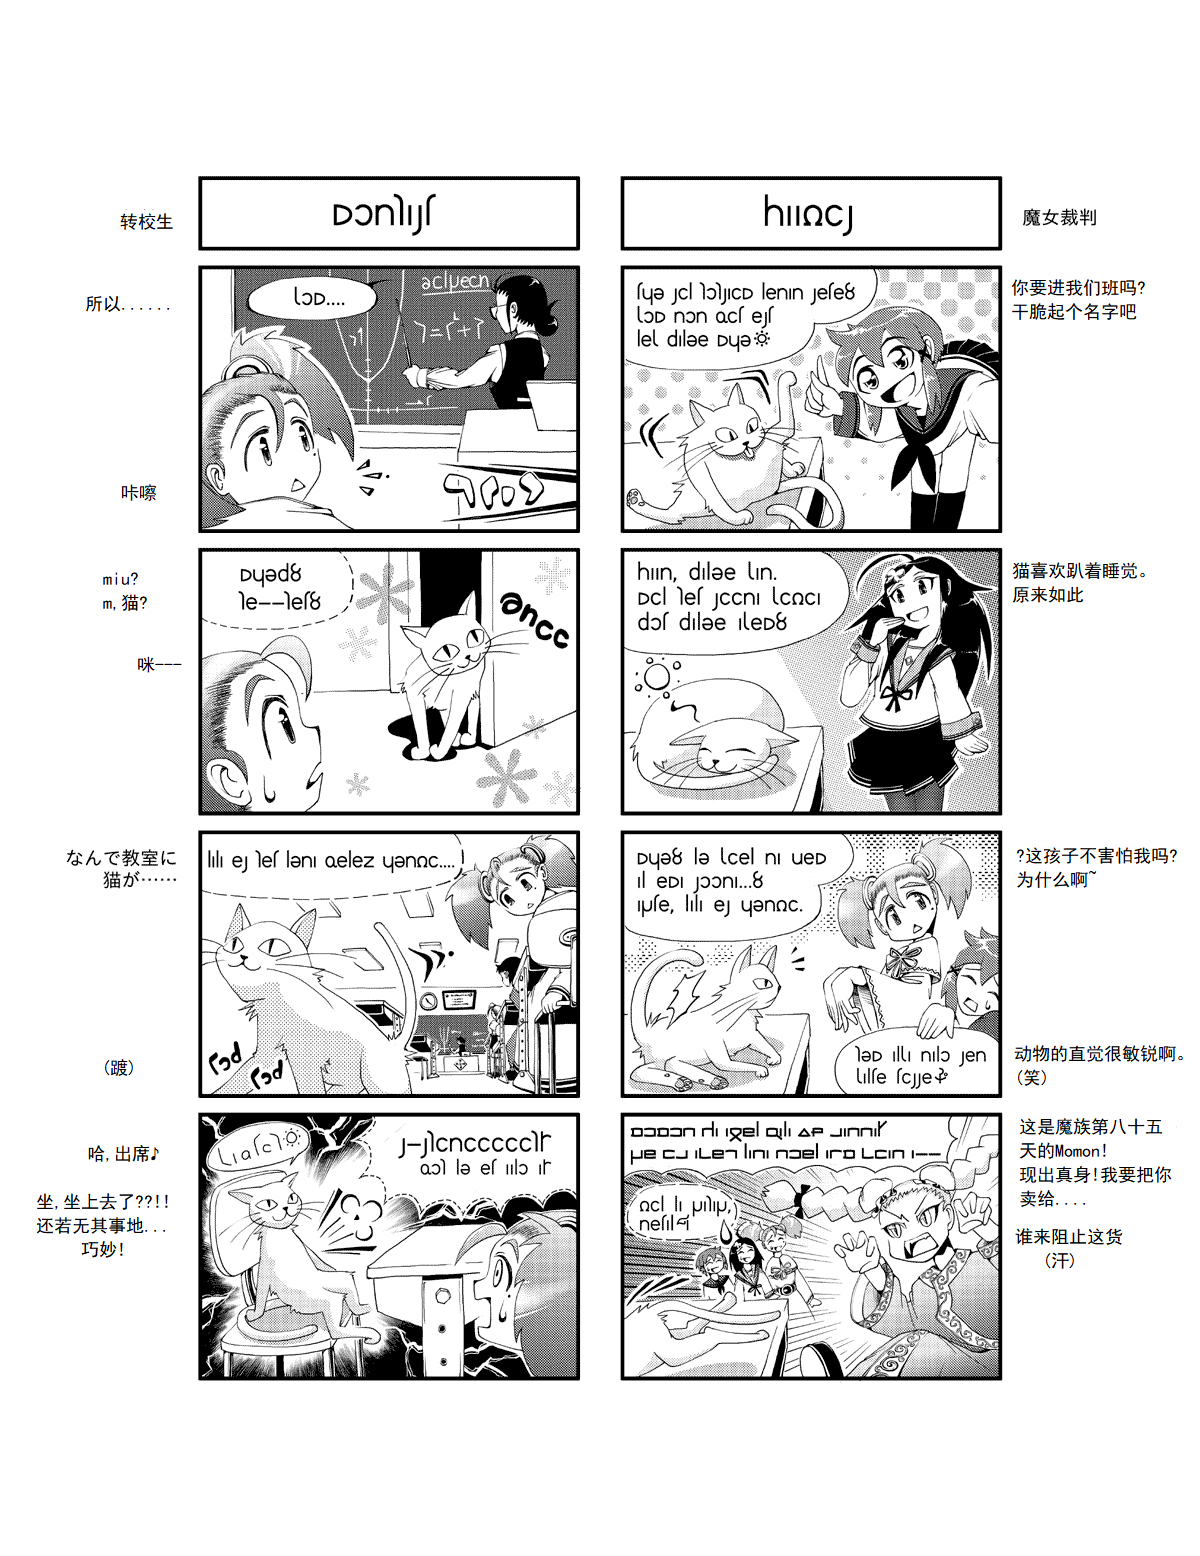
\includegraphics[width=\textwidth]{pngs/xarl2.png}%或者height=\textheight
\end{figure}



\emoji{x_nau} 
啊,是四格漫画呀,也有异世界呢♪


\emoji{l_rana} 

这是在中央Arna大学的四个女生的故事哦。名字叫「猫猫日记」。

4格漫画用起承转合的结构叙述,容易理解.从画面里也能看到文化和举止,意外地有学习性呢.

今天我们用右边的漫画,一格一格地读.

\emoji{a_nax} 
顺便说一下Arna大学就是我和Lein上的学校哦.

说是大学,对日本人来说也只是高中生吧.

lein在Lydia带的1班,我在Lardura带的八班.不知道这几个人在哪一班.


\emoji{l_ket} 
我觉得是猫班♪
